\begin{figure*}[t]
\centering
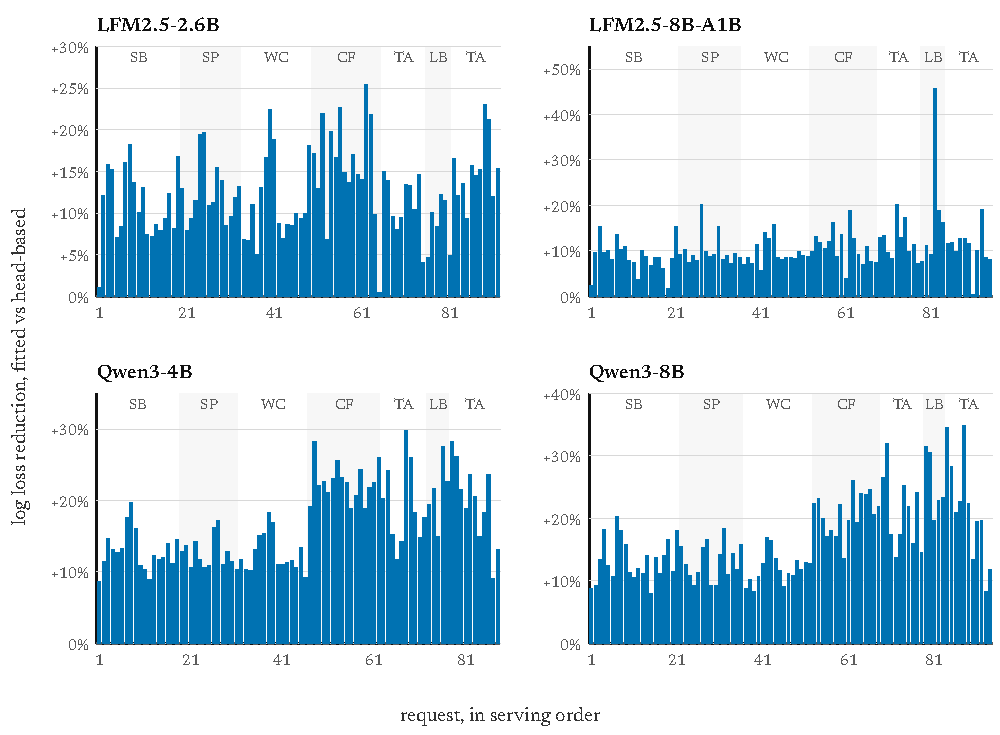
\includegraphics[width=0.8\textwidth]{gen/fig-accept-curve-img.pdf}
\caption{The acceptance model while serving the evaluation subset from an empty store (looped replies left out): for each request, how much lower the fitted model's log loss per labelled node is than that of the head-based estimate it competes with (1 $-$ fitted / head-based), both scored before either learns from the request's labels. A bar above the dashed zero line (blue) is a request the fitted model predicted better. Shaded bands mark the six sources in serving order (SB Spec-Bench, SP SPEED-Bench, WC WildChat, CF ConvFinQA, TA ToolACE, LB LongBench). The fitted model is lower on 91 of 91, 94 of 94, 87 of 87, 93 of 93 requests after the first, in the order of the panels. At the 20 changes of source (five on each target), the first request of the new source ranks 0.47 on average among that source's other requests by this reduction (0 lowest, 1 highest) and below their median at 8 of them.}
\label{fig:accept-curve}
\end{figure*}
